\documentclass[12pt,a4paper]{article}
\usepackage[english, science, large]{../template/ku-frontpage}
\usepackage{tabularx}
\usepackage{ltablex}
\usepackage[cache=false]{minted}
\setminted[erlang]{
frame=lines,
framesep=2mm,
baselinestretch=1.1,
fontsize=\footnotesize,
linenos,
breaklines}
\usemintedstyle{friendly}
\hypersetup{
    colorlinks=false,
    pdfborder={0 0 0},
}
\begin{document}

\title{Quizmaster}
\subtitle{Assignment 5}

\author{Kai Arne S. Myklebust, Silvan Adrian}
\date{Handed in: \today}
	
\maketitle
\tableofcontents

\section{Solution}

\subsection{Files}
All Files are situated in the \textbf{src/} folder:
\begin{itemize}
	\item \textbf{flamingo.erl} The flamingo server implmentation
	\item \textbf{greetings.erl} The greetings module implementation
	\item \textbf{hello.erl} The hello module implementation
	\item \textbf{mood.erl} Mood module implementation
	\item \textbf{counter.erl} Counter module implementation
	\item \textbf{test\_xxx.erl} Tests for each module
\end{itemize}

\subsection{Running the programm}
Out of convenience we used a Emakefile which compiles all the erlang files in one go then rather compile each file on it's own.
This can be done by using the erlang shell and run:

\begin{minted}{erlang}
make:all([load]).
\end{minted}

\subsection{Running the tests}
The tests can be run with eunit, we included tests for each module in a own file.
Example running tests for flamingo:
\begin{minted}{erlang}
eunit:test(test_flamingo, [verbose]).
\end{minted}

\section{Implementation}
\subsection{Gen-Statem}
Since the Quizmaster can be seen as a simple State machine we chose gen\_statem.
The Quizmaster has overall 3 important states:
\begin{itemize}
	\item editable
	\item between\_question
	\item active\_question
\end{itemize} 

\begin{figure}
\begin{center}
		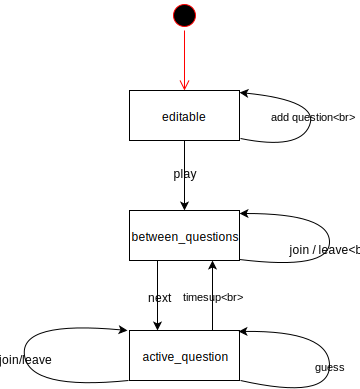
\includegraphics[width=0.8\textwidth]{images/Quizmaster}
\end{center}
	\caption{Simple drawing of quizmaster state machine}
\end{figure}

\subsection{Data Structure}


\subsection{Editable state}
\subsection{Between\_questions state}
\subsection{Active\_question state}

needs to be improved

\section{Assessment}

\subsection{Scope of Test Cases}

\subsection{Correctness}

\subsection{Code Quality}


\appendix
\section{Code Listing}

\end{document}}